\renewcommand\thechapter{\Roman{chapter}}
\chapter{MÉTODO} \label{ch:metodo} \thispagestyle{fancy}
\renewcommand\thechapter{\arabic{chapter}}
%%%%%%%%%%%%%%%%%%%%%%%%%%%%%%%%%%%%%%%%%%%%%%%%%%%%%%%%%%%%%%%%%%%%%%%%%%%%
En este capítulo se describe la ruta metodológica que se tomó para diseñar y desarrollar el coprocesador para la convolución. Primero, se indica el sujeto de estudio. Después, se muestra un diagrama de flujo con las etapas del proyecto, así como la descripción de cada una. Por último, se enlistan los materiales y herramientas utilizados.


\section{Sujeto}
\begin{itemize}
\item Investigadores e ingenieros del area de desarrollo de hardware y cómputo de alto rendimiento. 
\end{itemize}

\section{Procedimiento}

\begin{figure}[!h]
\centering
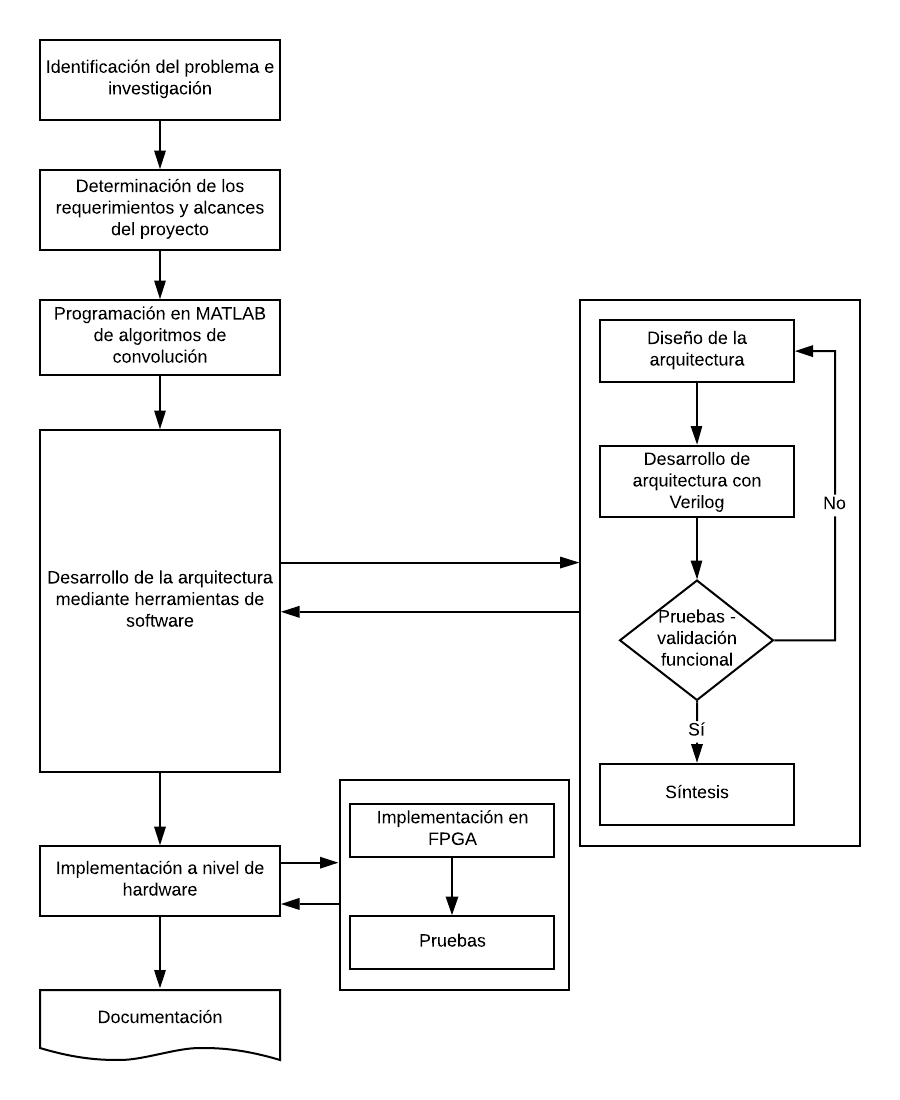
\includegraphics[width=1\textwidth, height=1\textheight]{./figs/procedimiento}\\
\caption{Diagrama de flujo}
\label{diagramaflujo}
\end{figure}

\newpage
En la figura \ref{diagramaflujo} se muestran los pasos que se siguieron para desarrollar el coprocesador para la convolución. A continuación, se describre cada una de las etapas del proyecto.

\subsection{Identificación del problema e investigación}
Se determina la problemática, en base al análisis del entorno actual de la computación, al cual se le buscará solución con el proyecto que se presenta en este trabajo. El problema que se aborda es la necesidad de encontrar alternativas a las tendencias actuales para el procesamiento de señales con mejores prestaciones de cómputo intensivo y con menor consumo de potencia, específicamente para la operación de la convolución.

Además, se recopila información acerca de trabajos similares en bases de datos de artículos científicos y en libros técnicos. Esta información sirve como punto de referencia para comparar el rendimiento de la arquitectura propuesta en este trabajo, además se analizan las áreas de oportunidades de estos trabajos para proponer una solución más óptima al problema planteado. En esta etapa se investiga cuál es la situación actual de la tecnología de cómputo de alto rendimiento la cual se describe en el estado del arte.

\subsection{Determinación de los requerimientos y alcances del proyecto}
Se determinan los requerimientos que se buscan satisfacer con el coprocesador desarrollado en este trabajo. Además, se indican cuáles son los alcances y delimitaciones del proyecto. Este trabajo se limitará a diseñar  la arquitectura de un coprocesador capaz de resolver la operación de la convolución de dos señales. Se implementará en un FPGA y se verificará a través de un entorno de simulación con la ayuda de MATLAB, donde se realizarán pruebas de rendimiento con respecto al tiempo de procesamiento. Las limitaciones del proyecto son el tiempo disponible, dinero, recursos y licencias.

\subsection{Programación en MATLAB de algoritmos de convolución}
Se programan diferentes algoritmos existentes para resolver la convolución utilizando MATLAB. El objetivo de esta etapa es comparar el rendimiento en tiempo de ejecución y uso de recursos de memoria de los diferentes algoritmos y analizar las ventajas y desventajas de cada uno de ellos. 

\subsection{Desarrollo de la arquitectura mediante herramientas de software}
Se desarrolla la arquitectura en un ambiente de software, haciendo uso de programas de software para descripción y simulación de la arquitectura, una metodología de diseño y un lenguaje de descripción de hardware. 

\subsubsection{Diseño de la arquitectura}
Mediante el uso de la metodología Top-Down y en base a las arquitecturas de la actualidad se desarrolla una arquitectura capaz de realizar la operación de la convolución con un menor consumo de potencia y con una velocidad de procesamiento comparable con las arquitecturas modernas.  

\subsubsection{Desarrollo de arquitectura con Verilog}
Con la ayuda de un lenguaje de descripción de hardware, en este caso Verilog, se describe la arquitectura digital en Xilinx ISE 14.7. Se describen los diferentes bloques que forman parte de la arquitectura, posteriormente se unen estos elementos con un top level para formar un sistema capaz de convolucionar dos señales.

\subsubsection{Pruebas - validación funcional}
Se simula la arquitectura mediante el uso de test benchs. Los resultados se comparan con resultados obtenidos con la función predeterminada de MATLAB llamada conv() la cual realiza la operación de la convolución de dos señales. En caso de no obtener los resultados esperados, se vuelve a diseñar la arquitectura. 

\subsubsection{Síntesis}
Se realiza la síntesis lógica del código, la cual consiste en convertir la descripción de hardware especificada mediante Verilog en una implementación de diseño en término de compuertas lógicas, la cual es un archivo de flujo de bits (.bit).  

\subsection{Implementación a nivel de hardware}
En esta etapa se programa el FPGA. Además, se realizan pruebas a la arquitectura propuesta para comprobar que se cumplen los requerimientos planteados al inicio del proyecto y para verificar que la operación de la convolución se realiza de manera correcta. 

\subsubsection{Implementación en FPGA}
Una vez que se cuenta con la arquitectura sintetizada, se programa el archivo de flujo de bits en el FPGA utilizando el software Digilent Adept. Este archivo le indica al FPGA cómo se tiene que configurar para realizar la operación de la convolución.

\subsubsection{Pruebas}
Se realizan pruebas al hardware mediante una interfaz de comunicación serial la cual conecta al FPGA con una PC. Se envian dos señales al FPGA, las cuales se convolucionan en la arquitectura digital, y este da como resultado una tercera señal la cual se envía a la PC. El resultado se compara con resultados obtenidos bajo un ambiente conocido en MATLAB y sirve para comprobar que el sistema digital está funcionando de manera correcta. Además, se realizan pruebas de velocidad de procesamiento y consumo de potencia para comparar con diferentes arquitecturas.

\subsection{Documentación}
Por último, se realiza un trabajo escrito en el cual se documentan los aspectos más relevantes del proyecto. Primero, se da una introducción al proyecto y se pone en contexto al lector, después se presenta el trabajo realizado así como se describe a detalle la forma en que se realizó cada etapa, posteriormente, se presentan los resultados obtenidos así como un análisis de los mismos, haciendo una comparación con las arquitecturas que ya están disponibles en el mercado, por último, se concluye y se proponen mejoras para trabajos futuros. 

\section{Materiales y Herramientas}
\begin{itemize}
\item Laptop Dell Inspiron 13-5378
\item MathWorks MATLAB R2015a
\item Xilinx ISE 14.7
\item Digilent Adept
\color{red}
\item agregar los que faltan (FPGA, OS(?))
\end{itemize}
